\section{Prueba 3: validación externa}
\label{cap:validacion-externa}

\subsection{Descripción} Se examinó la transferencia entre conjuntos y la degradación asociada al cambio de participante y de protocolo de adquisición.
La prueba responde tres preguntas: si WBCIC-SHU es un conjunto más difícil (se contrasta con un modelo
nativo), si la caída es un problema de escala de amplitud (la normalización por segmento la corregiría si fuese
una ganancia común a todos los canales) y cuánto de la caída corresponde a la persona y cuánto al protocolo
(protocolo de sujetos apartados).
\subsection{Procedimiento} Se armonizaron los canales y el preprocesamiento; se compararon los protocolos de la sección~\ref{sec:protocolos-extra} con las semillas 2026, 2027 y 2028.
\subsection{Resultados y análisis}


Al pasar de \openbmi{} a un conjunto registrado en otra institución, con otro amplificador y otro
montaje (el subconjunto de dos clases de WBCIC-SHU \cite{yang2025wbcic}, con $51$ participantes), la
exactitud de las cuatro arquitecturas cae entre $0.095$ y $0.123$ por el cambio de protocolo de adquisición.
El conjunto no es más difícil, la escala de amplitud no sostiene la explicación de la caída bajo el contraste
de normalización, y el diseño no permite afirmar que la caída por protocolo supere a la debida al cambio de
persona. Los protocolos son los de la
sección~\ref{sec:protocolos-extra} y el preprocesamiento se armonizó según la
sección~\ref{sec:wbcic-preproc}. Los resultados son la media de tres semillas ($2026$, $2027$ y $2028$), con
la desviación típica entre semillas cuando procede, y los diez sujetos apartados son los mismos en las tres;
los resultados con alineamiento euclidiano proceden de la semilla $2026$.

La evaluación aborda la carencia de evaluaciones estandarizadas de los modelos fundacionales de EEG
\cite{kuruppu2026fmreview}: el conjunto externo no figura en las fuentes de preentrenamiento declaradas de
LaBraM (sección~\ref{sec:limitaciones}), las cuatro arquitecturas se evalúan con el mismo protocolo,
preprocesamiento y segmentos de prueba, y el protocolo de sujetos apartados
(sección~\ref{sec:descomposicion}) separa la degradación por persona de la debida al protocolo de
adquisición, que una evaluación fuera de distribución convencional confunde en una sola cifra. El
protocolo de adquisición es aquí un factor compuesto (institución, amplificador, montaje y $45$ canales
comunes, población, una sola sesión y diferencias de preprocesamiento no igualables,
tabla~\ref{tab:armonizacion}), y la descomposición atribuye la caída a ese conjunto sin separar sus
componentes.

\subsection{Transferencia \textit{zero-shot} frente a un modelo nativo}

\textbf{WBCIC-SHU no es un conjunto más difícil}: un modelo entrenado sobre él alcanza entre $0.766$ y
$0.822$, mientras que el modelo transferido desde \openbmi{} sin reentrenar alcanza entre $0.596$ y $0.620$
(tabla~\ref{tab:transferencia}). Ambos se miden sobre \textbf{los mismos $2\,040$ segmentos reservados}; el
transferido se entrenó con los $54$ sujetos de \openbmi{} y el nativo con los $51$ de WBCIC-SHU.

\begin{table}[H]
\centering
\caption{Transferencia \textit{zero-shot} desde \openbmi{} frente a un modelo entrenado en
WBCIC-SHU, ambos evaluados sobre los mismos $2\,040$ segmentos reservados. Media de las tres
semillas $\pm$ desviación típica entre semillas, que con tres valores es una estimación gruesa.
Azar $0.50$. El modelo transferido emplea la política de normalización \emph{origen}, fijada de
antemano y empleada también en la tabla~\ref{tab:descomposicion}; las otras dos figuran en la
tabla~\ref{tab:politicas}. La última columna es la diferencia de la semilla $2026$ sola.}
\label{tab:transferencia}
\small
\begin{tabular}{lcccc}
\toprule
 & \textbf{Transferido} & \textbf{Nativo} & \textbf{Diferencia} & Diferencia 2026 \\
\midrule
\eegnet{} & $0.620 \pm 0.005$ & $0.812 \pm 0.004$ & $0.192 \pm 0.009$ & 0.182 \\
LaBraM & $0.610 \pm 0.007$ & $0.822 \pm 0.008$ & $0.212 \pm 0.014$ & 0.201 \\
Conformer & $0.614 \pm 0.003$ & $0.799 \pm 0.002$ & $0.185 \pm 0.005$ & 0.190 \\
EEGMamba & $0.596 \pm 0.006$ & $0.766 \pm 0.008$ & $0.169 \pm 0.007$ & 0.173 \\
\bottomrule
\end{tabular}
\end{table}

La exactitud del nativo es comparable a la del modelo global de \openbmi{} sobre sus propios sujetos vistos
($0.755$ a $0.819$), aunque esa medida es optimista porque se obtiene sobre el conjunto que determina la
parada temprana. La señal es decodificable; lo que no se logra es la transferencia. El orden entre las tres
primeras arquitecturas en la exactitud del transferido ($0.620$, $0.614$ y $0.610$) no es estable, porque sus
diferencias (de $0.004$ a $0.010$) son del orden de la desviación entre semillas ($0.003$ a $0.007$). La
diferencia entre nativo y transferido va de $0.169$ a $0.212$ y no lleva inferencia por participante, pues el
nativo no tiene valor por participante.

Dos sesgos de signo opuesto impiden leer esa diferencia como cota: el nativo \textbf{se entrenó con datos de
los $51$ sujetos}, es decir, sobre sujetos vistos, lo que aumenta la diferencia aparente; y entrena con $144$
segmentos por persona frente a $360$ de un modelo de \openbmi{}
(sección~\ref{sec:protocolos-extra}), lo que la reduce. No se ha medido cuál domina. La
sección~\ref{sec:descomposicion} obtiene una medida que no depende del modelo nativo.

\subsection{La caída no es un problema de escala}

La escala de amplitud \textbf{no sostiene la explicación de la caída}: la normalización por segmento, que
corregiría una ganancia global, no supera a la política \emph{origen}, que no usa ningún dato del destino
(tabla~\ref{tab:politicas}).

\begin{table}[H]
\centering
\caption{Exactitud del modelo transferido sobre el conjunto reservado de WBCIC-SHU según la
normalización aplicada al destino. Media de las tres semillas y de los $51$ sujetos. Azar
$0.50$. En negrita, la política de mayor media por arquitectura. Los contrastes pareados figuran
en la tabla~\ref{tab:politicas-contrastes}.}
\label{tab:politicas}
\small
\begin{tabular}{lccc}
\toprule
 & \textbf{Origen} & \textbf{Por segmento} & \textbf{Por sujeto} \\
\midrule
\eegnet{} & \textbf{0.620} & 0.604 & 0.603 \\
LaBraM & \textbf{0.610} & 0.596 & 0.606 \\
Conformer & \textbf{0.614} & 0.578 & 0.593 \\
EEGMamba & 0.596 & 0.592 & \textbf{0.604} \\
\bottomrule
\end{tabular}
\end{table}

\begin{table}[H]
\centering
\caption{Contrastes pareados por participante (51) de la política \emph{origen} frente a cada
alternativa, con la exactitud promediada entre las tres semillas dentro de cada participante.
Intervalo de percentiles del remuestreo de participantes. Corrección de Holm sobre los ocho
contrastes.}
\label{tab:politicas-contrastes}
\small
\begin{tabular}{llcccc}
\toprule
 & Contraste & Dif. & IC $95$\,\% & $p$ & $p_{\text{Holm}}$ \\
\midrule
\eegnet{} & origen $-$ segmento & $+0.016$ & $[+0.007,\ +0.024]$ & 0.001 & 0.010 \\
\eegnet{} & origen $-$ sujeto & $+0.017$ & $[+0.004,\ +0.032]$ & 0.061 & 0.24 \\
LaBraM & origen $-$ segmento & $+0.014$ & $[+0.004,\ +0.025]$ & 0.015 & 0.091 \\
LaBraM & origen $-$ sujeto & $+0.004$ & $[-0.008,\ +0.017]$ & 0.72 & 1.00 \\
Conformer & origen $-$ segmento & $+0.036$ & $[+0.019,\ +0.052]$ & $<0.001$ & 0.001 \\
Conformer & origen $-$ sujeto & $+0.021$ & $[+0.006,\ +0.036]$ & 0.036 & 0.18 \\
EEGMamba & origen $-$ segmento & $+0.004$ & $[-0.005,\ +0.014]$ & 0.71 & 1.00 \\
EEGMamba & origen $-$ sujeto & $-0.008$ & $[-0.021,\ +0.005]$ & 0.26 & 0.77 \\
\bottomrule
\end{tabular}
\end{table}

Las tres políticas caen dentro de $1.7$ puntos entre sí en \eegnet{}, LaBraM y EEGMamba, y en el
Conformer dentro de $3.6$. El origen es la mejor en tres de las cuatro arquitecturas y, tras la corrección
de Holm sobre los ocho contrastes, supera a la normalización por segmento en \eegnet{}
($p_{\text{Holm}} = 0.010$) y en el Conformer ($0.001$); en EEGMamba la media mayor es la de la
normalización por sujeto y la diferencia no se detecta ($p_{\text{Holm}} = 0.77$). Usar estadísticos del
destino antes de clasificar no aporta una mejora consistente.

El alcance es limitado: la política por segmento solo elimina la escala global del segmento, y las
alternativas se aplican a un modelo entrenado con los estadísticos del origen, por lo que el contraste no
distingue entre que la escala no sea la causa y que el modelo no tolere otra normalización. Ninguna de las
políticas corrige diferencias de covarianza espacial, que un alineamiento de covarianzas abordaría
\cite{he2020ea,zanini2018} (sección~\ref{sec:ea-transferencia}).

\subsection{Descomposición de la degradación entre persona y protocolo}
\label{sec:descomposicion}

La \textbf{caída por cambio de protocolo} es clara: se sitúa entre $0.095$ y $0.123$ y su intervalo excluye
el cero en las cuatro arquitecturas. La caída por cambio de persona es menor en estimación puntual (de
$0.055$ a $0.087$), pero se estima con mucha menos precisión, y \textbf{la diferencia entre ambas caídas no
es significativa} en ninguna arquitectura (tablas~\ref{tab:descomposicion} y~\ref{tab:descomposicion-ic}).
Las tres columnas de desempeño proceden de un mismo conjunto de pesos por arquitectura y semilla, entrenado
con $44$ sujetos y los $45$ canales comunes, de modo que sus diferencias son restables; la segunda diferencia
corresponde al factor compuesto del protocolo de adquisición. La columna de sujetos vistos es el conjunto
que determina la parada temprana y comparte sesión con el entrenamiento, lo que tiende a elevar la caída
atribuida a la persona.

\begin{table}[H]
\centering
\caption{Descomposición del cambio de dominio con el protocolo de sujetos apartados. Media de
las tres semillas; las tres primeras columnas son el mismo modelo evaluado en tres conjuntos. En las dos
últimas columnas, $\pm$ es la desviación típica entre las tres semillas. Normalización
\emph{origen}. Azar $0.50$. Los intervalos de las caídas figuran en la
tabla~\ref{tab:descomposicion-ic}.}
\label{tab:descomposicion}
\small
\begin{tabular}{lccccc}
\toprule
 & \multicolumn{3}{c}{\textbf{Exactitud}} & \multicolumn{2}{c}{\textbf{Caída atribuible a}} \\
\cmidrule(lr){2-4}\cmidrule(lr){5-6}
 & Vistos & Persona nueva & WBCIC-SHU & Persona & Protocolo \\
\midrule
\eegnet{} & 0.793 & 0.738 & 0.623 & $0.055 \pm 0.005$ & $0.115 \pm 0.006$ \\
Conformer & 0.810 & 0.722 & 0.618 & $0.087 \pm 0.008$ & $0.104 \pm 0.014$ \\
LaBraM & 0.811 & 0.739 & 0.616 & $0.071 \pm 0.004$ & $0.123 \pm 0.006$ \\
EEGMamba & 0.755 & 0.692 & 0.598 & $0.062 \pm 0.020$ & $0.095 \pm 0.010$ \\
\bottomrule
\end{tabular}
\end{table}

La columna \emph{persona nueva} se estima sobre $10$ sujetos y la de WBCIC-SHU sobre $51$, con desviaciones
típicas entre sujetos de $0.095$ a $0.129$ y de $0.096$ a $0.124$. Los intervalos de la
tabla~\ref{tab:descomposicion-ic} son de percentiles por remuestreo jerárquico de los sujetos apartados, los
de WBCIC-SHU y sus semillas ($B = 10\,000$), con la exactitud de los sujetos vistos ($1\,760$ ensayos)
como fija. Sus límites varían en la tercera cifra según la variante del intervalo, de modo que los que
quedan a menos de $0.005$ de cero no permiten decidir si lo incluyen, y con solo $10$ sujetos apartados
pueden subestimar la incertidumbre.

\begin{table}[H]
\centering
\caption{Intervalos de confianza al $95$\,\% de las caídas de la
tabla~\ref{tab:descomposicion}, por remuestreo jerárquico de los sujetos apartados, los de
WBCIC-SHU y sus tres semillas. La última columna es la diferencia entre la caída por protocolo y la caída por
persona.}
\label{tab:descomposicion-ic}
\footnotesize
\setlength{\tabcolsep}{4pt}
\begin{tabular}{lccc}
\toprule
 & \textbf{Caída por persona} & \textbf{Caída por protocolo} & \textbf{Protocolo $-$ persona} \\
\midrule
\eegnet{} & $0.055\ [-0.019,\ +0.126]$ & $0.115\ [+0.035,\ +0.195]$ & $0.060\ [-0.085,\ +0.212]$ \\
Conformer & $0.087\ [+0.007,\ +0.161]$ & $0.104\ [+0.022,\ +0.193]$ & $0.017\ [-0.134,\ +0.183]$ \\
LaBraM & $0.071\ [+0.006,\ +0.135]$ & $0.123\ [+0.050,\ +0.198]$ & $0.052\ [-0.082,\ +0.187]$ \\
EEGMamba & $0.062\ [-0.001,\ +0.120]$ & $0.095\ [+0.034,\ +0.161]$ & $0.032\ [-0.082,\ +0.159]$ \\
\bottomrule
\end{tabular}
\end{table}

Que el intervalo de la caída por persona incluya o no el cero depende de la variante del intervalo (en
\eegnet{} lo incluye siempre, en el Conformer lo excluye siempre, y en LaBraM y EEGMamba depende de la
variante, con límites a menos de $0.002$ del cero en EEGMamba con tres semillas). Las cuatro estimaciones
puntuales de la diferencia entre ambas caídas son positivas, la del Conformer ($0.017$) la menor, y las del
Conformer y EEGMamba son muy variables entre semillas (de $0.003$ a $0.041$ y de $-0.002$ a $0.050$).

La caída por persona es mayor aquí que en \loso{} en las cuatro arquitecturas, entre $1.7$ y $3.1$ veces
($0.020$ a $0.041$ en \loso{}); la razón es descriptiva, porque las cifras proceden de modelos distintos. A
la discrepancia pueden contribuir cuatro diferencias que el diseño no separa: la estimación descansa en $10$
sujetos frente a $54$; la columna de vistos es el conjunto que determina la parada temprana
(sección~\ref{sec:dsi}); los modelos usan $45$ canales frente a $62$; y los diez sujetos apartados rinden
algo por debajo del resto en \loso{} (sección~\ref{sec:protocolos-extra}). La estimación de \loso{}, más
precisa, es coherente con las puntuales: sus intervalos jerárquicos al $95$\,\% tienen como límite superior
entre $0.053$ y $0.070$, por debajo de la caída por protocolo; se presenta como indicio y no como contraste,
porque procede de otros modelos y de otro número de canales.

Así, el \dsi{} (subsección~\ref{sec:dsi-resultados}), positivo en las cuatro entre $+0.026$ y $+0.052$ y con
límites superiores de $0.068$ a $0.088$ (tabla~\ref{tab:bootstrap}), mide la degradación ante personas nuevas del mismo conjunto; la validación
externa añade la caída al cambiar de conjunto de datos, que ese indicador no proporciona.

\subsection{Aplicación del criterio de robustez}
\label{sec:aplicacion-robustez}

\textbf{Ninguna arquitectura domina los tres ejes del criterio de robustez}, y las diferencias entre ellas
quedan por debajo de la incertidumbre de la estimación (tabla~\ref{tab:robustez}). El \dsi{} procede de
\loso{} y el \idp{} del protocolo de sujetos apartados (ecuaciones~\eqref{eq:dsi} y~\eqref{eq:idp});
las columnas de estabilidad se calculan sobre las exactitudes \loso{} promediadas por participante.

\begin{table}[H]
\centering
\caption{Los tres ejes del criterio de robustez, con la media de tres semillas por participante.
Menor es mejor en las columnas de
degradación, en la desviación típica (Desv.) y en el recuento bajo umbral; mayor es mejor en la exactitud y en el percentil
$5$. Ninguna arquitectura obtiene el mejor valor en los tres ejes.}
\label{tab:robustez}
\small
\begin{tabular}{lcccccc}
\toprule
 & \multicolumn{2}{c}{\textbf{Degradación}} & \multicolumn{3}{c}{\textbf{Estabilidad entre participantes}} & \\
\cmidrule(lr){2-3}\cmidrule(lr){4-6}
 & \dsi{} & \idp{} & Desv. & Percentil 5 & Bajo $0.70$ & Exactitud \loso{} \\
\midrule
\eegnet{} & \textbf{0.026} & 0.156 & 0.119 & 0.562 & 17/54 & \textbf{0.761} \\
Conformer & 0.037 & 0.144 & 0.121 & 0.555 & 19/54 & 0.747 \\
LaBraM & 0.052 & 0.167 & 0.107 & \textbf{0.581} & \textbf{15/54} & 0.755 \\
EEGMamba & 0.036 & \textbf{0.137} & \textbf{0.103} & 0.552 & 26/54 & 0.715 \\
\bottomrule
\end{tabular}
\end{table}

El menor \dsi{} corresponde a \eegnet{}, el menor \idp{} a EEGMamba ($0.137$, frente a $0.144$ del Conformer,
diferencia menor que la desviación entre semillas de este último, $0.018$) y el menor recuento bajo umbral a
LaBraM, que tiene además la mayor caída por protocolo ($0.123$) y el percentil $5$ más alto ($0.581$).
EEGMamba presenta la menor desviación ($0.103$), pero queda por debajo en exactitud y en recuento bajo umbral
y tiene el percentil $5$ más bajo ($0.552$), el caso de compresión del rango advertido en la definición del
criterio. La diferencia entre las caídas por protocolo y por persona del Conformer vale $0.003$, $0.007$ y
$0.041$ en las tres semillas, y la de EEGMamba $0.048$, $0.050$ y $-0.002$, de modo que ningún patrón del
Conformer es exclusivo ni estable.

El \idp{} es entre $3.2$ y $6.1$ veces el \dsi{}, una proporción solo descriptiva, porque proceden de
protocolos distintos ($62$ frente a $45$ canales); la comparación del mismo modelo sobre los mismos canales es
la de la sección~\ref{sec:descomposicion}. De ello no se sigue que alguna sea más robusta: el \idp{} se
sitúa entre $0.137$ y $0.167$ pese a diferir hasta en tres órdenes de magnitud en parámetros, en el
preentrenamiento y en el procesamiento de la señal. Sus intervalos jerárquicos al $95$\,\% son $[0.054,\
0.243]$ (\eegnet{}), $[0.034,\ 0.242]$ (Conformer), $[0.074,\ 0.248]$ (LaBraM) y $[0.054,\ 0.215]$ (EEGMamba),
de amplitud $0.16$ a $0.21$. Que arquitecturas de $2\,626$ parámetros y de $5.8$ millones presenten caídas no
distinguibles es compatible con que el factor limitante no sea una dimensión de diseño explorada aquí, sin que
el diseño permita establecerlo. Las cuatro comparten la señal en el dominio del tiempo como espacio de
predicción, por lo que la representación permanece constante en la comparación (véase la discusión).

\subsection{Alineamiento euclidiano en la transferencia}
\label{sec:ea-transferencia}

El alineamiento euclidiano \textbf{no recupera la caída por protocolo}: la caída calculada aumenta en las
cuatro arquitecturas (de $+0.033$ a $+0.068$), con intervalo que excluye el cero en \eegnet{} y en EEGMamba
(tablas~\ref{tab:ea-transferencia} y~\ref{tab:ea-caidas}). El contraste es pareado por participante frente a
la base de la misma semilla ($2026$), con los $45$ canales comunes; al ser una sola semilla, el cambio se
compara como orden de magnitud con la desviación entre semillas de la base ($0.004$ a $0.007$).

\begin{table}[H]
\centering
\caption{Variante con alineamiento euclidiano menos la base de la misma semilla ($2026$), por evaluación:
modelo de $54$ sujetos evaluado en WBCIC-SHU, y modelo de $44$ sujetos evaluado en WBCIC-SHU y en los $10$
sujetos apartados. $p_{\text{Holm}}$ sobre los doce contrastes.}
\label{tab:ea-transferencia}
\footnotesize
\resizebox{\textwidth}{!}{%
\begin{tabular}{llcccc}
\toprule
\textbf{Arq.} & \textbf{Evaluación} & Base 2026 & EA 2026 & Dif., IC $95$\,\% & $p_{\text{Holm}}$ \\
\midrule
\eegnet{} & 54 $\to$ WBCIC-SHU & 0.626 & 0.632 & $+0.006$ $[-0.018,\ +0.028]$ & 1.00 \\
 & 44 $\to$ WBCIC-SHU & 0.621 & 0.610 & $-0.011$ $[-0.034,\ +0.012]$ & 1.00 \\
 & 44 $\to$ 10 apartados & 0.742 & 0.799 & $+0.057$ $[+0.022,\ +0.093]$ & 0.17 \\
\midrule
Conformer & 54 $\to$ WBCIC-SHU & 0.611 & 0.622 & $+0.011$ $[-0.012,\ +0.036]$ & 1.00 \\
 & 44 $\to$ WBCIC-SHU & 0.618 & 0.630 & $+0.012$ $[-0.008,\ +0.032]$ & 1.00 \\
 & 44 $\to$ 10 apartados & 0.718 & 0.763 & $+0.045$ $[+0.013,\ +0.078]$ & 0.37 \\
\midrule
LaBraM & 54 $\to$ WBCIC-SHU & 0.613 & 0.623 & $+0.009$ $[-0.007,\ +0.026]$ & 1.00 \\
 & 44 $\to$ WBCIC-SHU & 0.628 & 0.595 & $-0.033$ $[-0.059,\ -0.006]$ & 0.28 \\
 & 44 $\to$ 10 apartados & 0.745 & 0.748 & $+0.003$ $[-0.030,\ +0.032]$ & 1.00 \\
\midrule
EEGMamba & 54 $\to$ WBCIC-SHU & 0.589 & 0.598 & $+0.009$ $[-0.014,\ +0.032]$ & 1.00 \\
 & 44 $\to$ WBCIC-SHU & 0.598 & 0.600 & $+0.002$ $[-0.024,\ +0.027]$ & 1.00 \\
 & 44 $\to$ 10 apartados & 0.700 & 0.759 & $+0.060$ $[+0.033,\ +0.089]$ & 0.023 \\
\bottomrule
\end{tabular}
}
\end{table}

La causa numérica es que el alineamiento sube la exactitud de las personas nuevas de \openbmi{} (\eegnet{}
$+0.057$, Conformer $+0.045$, EEGMamba $+0.060$, LaBraM $+0.003$) y no la de WBCIC-SHU ($-0.011$, $+0.012$,
$+0.002$ y $-0.033$). Solo sobrevive a Holm el contraste de EEGMamba en las personas nuevas de \openbmi{}
($n = 10$, $p_{\text{Holm}} = 0.023$); en WBCIC-SHU ningún contraste es significativo. En la transferencia del
modelo de $54$ sujetos el cambio es de $+0.006$ a $+0.011$.

\begin{table}[H]
\centering
\caption{Variante con alineamiento euclidiano menos la base de la semilla $2026$, para las cantidades de la
descomposición, con intervalo al $95$\,\% del remuestreo pareado de los mismos participantes en las dos
variantes. Persona nueva: $10$ sujetos apartados; WBCIC-SHU (44): $51$ sujetos.}
\label{tab:ea-caidas}
\footnotesize
\resizebox{\textwidth}{!}{%
\begin{tabular}{lcccc}
\toprule
 & Persona nueva & WBCIC-SHU (44) & Caída por protocolo & Protocolo $-$ persona \\
\midrule
\eegnet{} & $+0.057$ $[+0.022,\ +0.093]$ & $-0.011$ $[-0.035,\ +0.013]$ & $+0.068$ $[+0.025,\ +0.111]$ & $+0.103$ $[+0.030,\ +0.180]$ \\
Conformer & $+0.045$ $[+0.013,\ +0.078]$ & $+0.012$ $[-0.009,\ +0.033]$ & $+0.033$ $[-0.006,\ +0.072]$ & $+0.052$ $[-0.016,\ +0.120]$ \\
LaBraM & $+0.003$ $[-0.030,\ +0.032]$ & $-0.033$ $[-0.060,\ -0.006]$ & $+0.036$ $[-0.007,\ +0.076]$ & $+0.012$ $[-0.060,\ +0.075]$ \\
EEGMamba & $+0.060$ $[+0.033,\ +0.089]$ & $+0.002$ $[-0.024,\ +0.027]$ & $+0.058$ $[+0.021,\ +0.097]$ & $+0.068$ $[+0.008,\ +0.133]$ \\
\bottomrule
\end{tabular}
}
\end{table}

Esto es compatible con que la caída por protocolo no sea un problema de covarianza espacial global, o con que
un alineamiento por participante con la covarianza media sea insuficiente; el diseño no separa ambas
explicaciones. El alineamiento es transductivo, por lo que estas cifras no son una transferencia
\textit{zero-shot} estricta, y el \eegnet{} con alineamiento entrenó más épocas que las bases, un régimen de
parada que no se separa del efecto del alineamiento.


\subsection{Comportamiento del entrenamiento}
\label{sec:curvas}

LaBraM y EEGMamba muestran sobreajuste y \eegnet{} y el Conformer apenas se separan
(figura~\ref{fig:curvas}). La figura muestra la evolución de la pérdida de las cuatro arquitecturas en los
dos protocolos de modelo único de la sección~\ref{sec:protocolos-extra}, que difieren en el volumen de
entrenamiento ($19\,440$ segmentos frente a $7\,342$).

\begin{figure}[H]
\centering
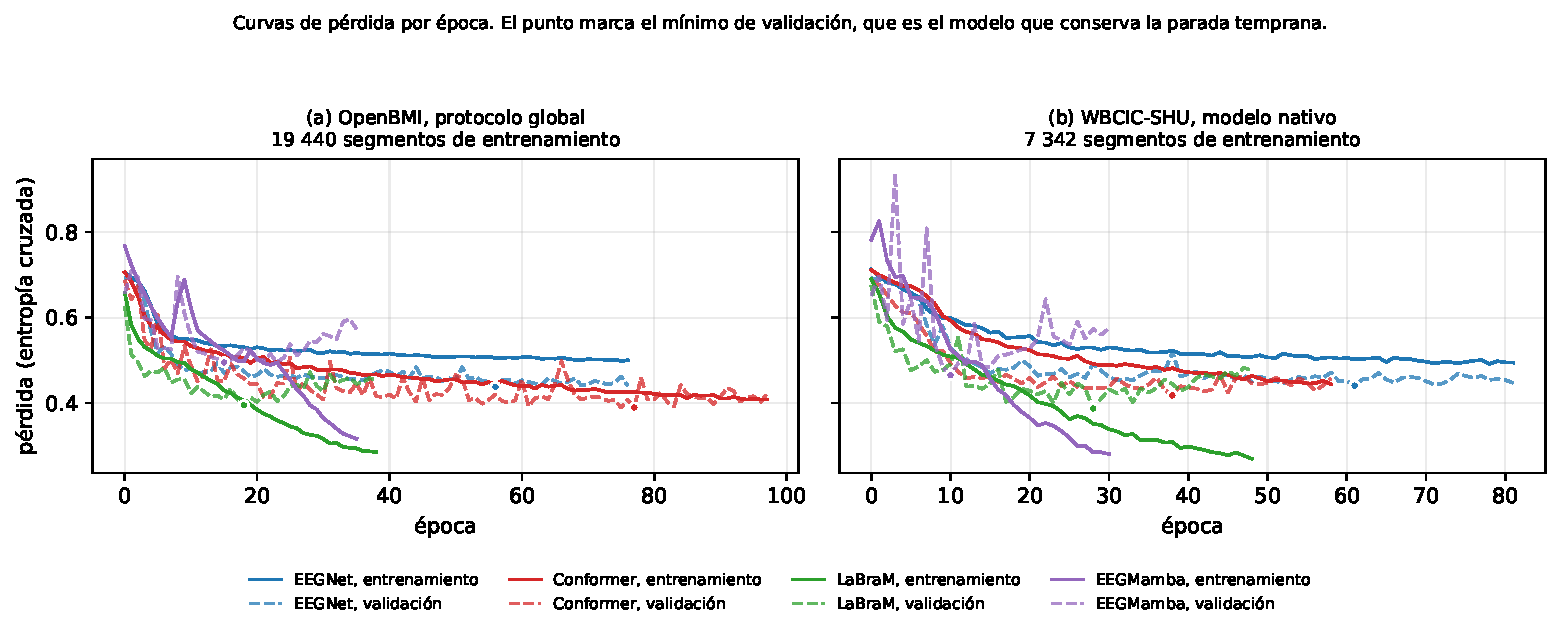
\includegraphics[width=\textwidth]{curvas_perdida.pdf}
\caption{Pérdida de entrenamiento (línea continua) y de validación (discontinua) por época.
(a) \openbmi{}, protocolo global sobre 54 sujetos. (b) WBCIC-SHU, modelo nativo sobre 51
sujetos, con menos de la mitad de segmentos de entrenamiento. El punto marca el mínimo de
validación, que es el modelo que conserva la parada temprana; las épocas posteriores no
forman parte del modelo evaluado.}
\label{fig:curvas}
\end{figure}

En LaBraM y EEGMamba la pérdida de entrenamiento queda por debajo de la de validación sin que esta última
mejore. El orden no sigue el número de parámetros (EEGMamba, con $3.4$ millones, se separa más que LaBraM,
con $5.8$). Los mínimos de validación del panel (a) se sitúan entre $0.39$ y $0.50$. Del panel (a) al (b)
el mínimo se alcanza antes en el Conformer y en EEGMamba, y la oscilación de la validación aumenta en tres de
las cuatro arquitecturas, de forma marcada en EEGMamba. Dos curvas de un único modelo por conjunto no bastan
para atribuir al volumen de datos la parada en las primeras épocas del protocolo intra-sujeto
(subsección~\ref{sec:seleccion-intra}).

\subsection{Referencias externas disponibles}

No hay cifras publicadas de clasificación entre sujetos sobre WBCIC-SHU con las que contrastar estos
resultados. Los autores del conjunto reportan, con validación cruzada de 10 \textit{folds} por sesión,
$0.853$ con \eegnet{} (media de las $153$ sesiones) y $0.818$ en la primera sesión \cite{yang2025wbcic}.
Aunque el protocolo difiere, el modelo nativo obtenido aquí, entre $0.766$ y $0.822$, es coherente con la
cifra de la primera sesión pese a entrenar con menos datos por persona.

